%%%%%%%%%%%%%%%%%%%%%%%%%%%%%%%%%%%%%%%%%%%%%%%%%%%%%%%%%%%%%%%%%%%%%
%%%%%%%%%%%%%%%%%%%%%%%%%%%%%%%%%%%%%%%%%%%%%%%%%%%%%%%%%%%%%%%%%%%%%
\begin{frame}{Decoupled architecture: Consensus/ Formation control}
	\begin{figure}
		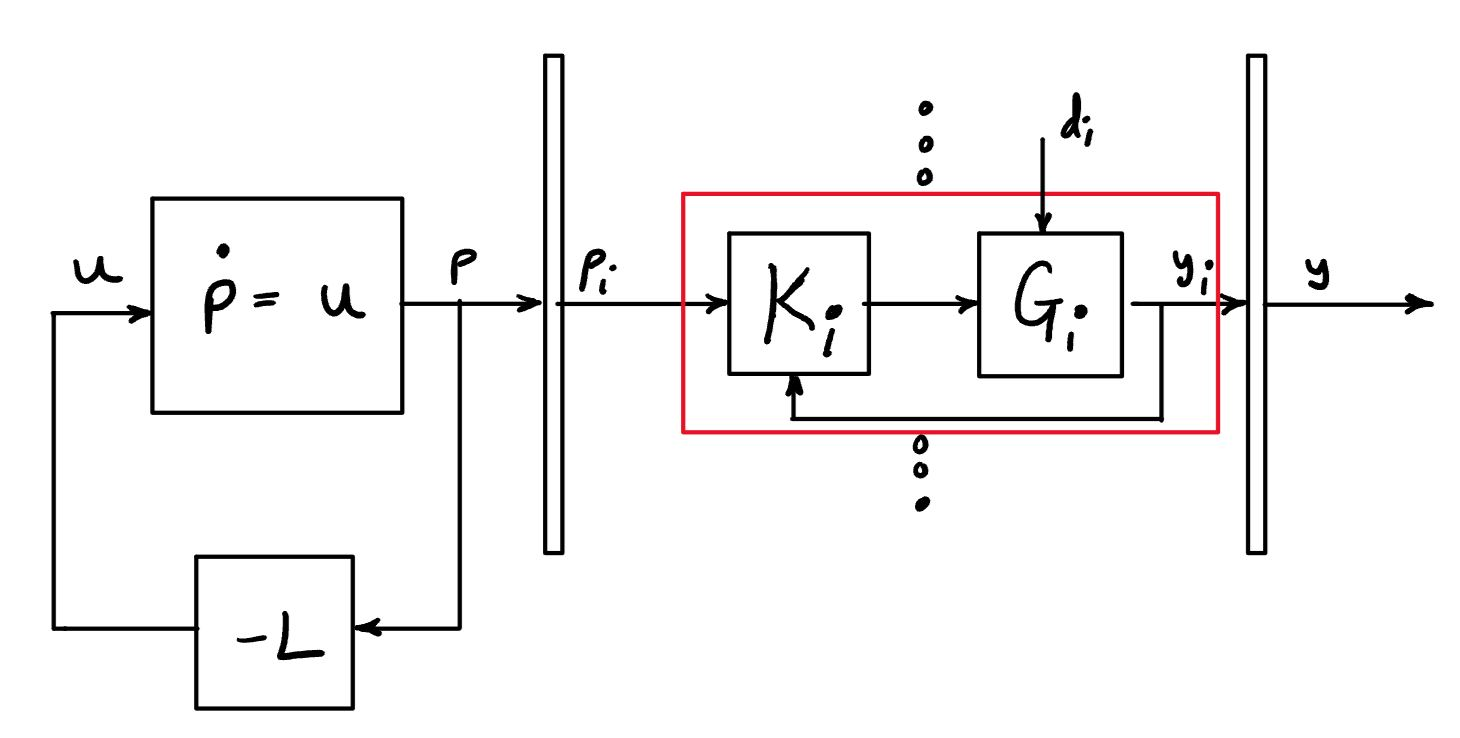
\includegraphics[scale=0.35]{figures/decoupled_consensus.JPG}	
		\label{fig:Coupled}
	\end{figure}
	\begin{itemize}
		\item Some related work
		\begin{itemize}
			\item Idea of wrapping local controllers around first order dynamics \footnote{Egerstedt and Cortes,2017}
			\item Combine a cooperation module with consensus moduke \footnote{Chen and Ren, 2019}
			\item Discrete-time Information flow filter \footnote{Fax and Murray, 2004}
		\end{itemize}
	\end{itemize}
\end{frame}
%%%%%%%%%%%%%%%%%%%%%%%%%%%%%%%%%%%%%%%%%%%%%%%%%%%%%%%%%%%%%%%%%%%%%
%%%%%%%%%%%%%%%%%%%%%%%%%%%%%%%%%%%%%%%%%%%%%%%%%%%%%%%%%%%%%%%%%%%%%
\begin{frame}{Decoupled architecture: Formation forming}	
		\begin{figure}
		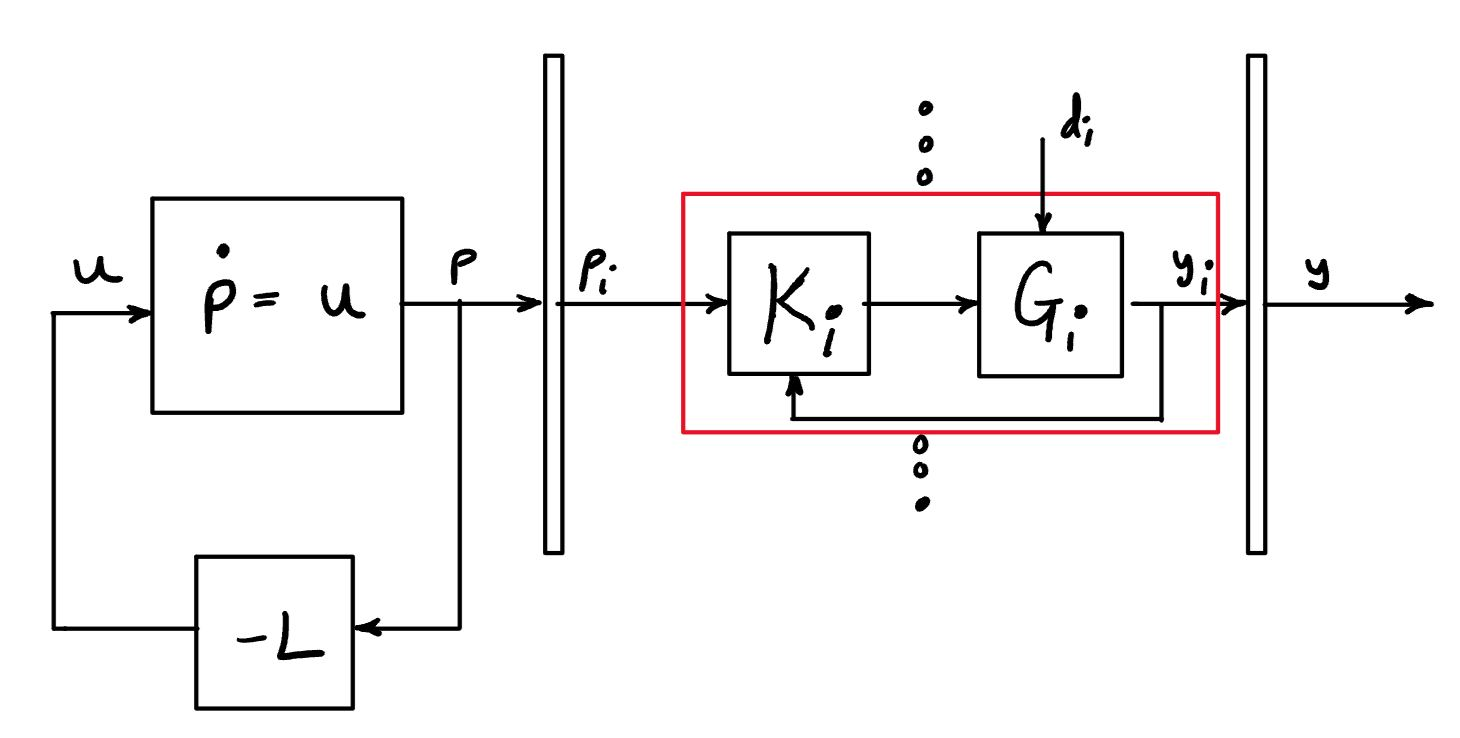
\includegraphics[scale=0.35]{figures/decoupled_consensus.JPG}	
		\label{fig:Coupled}
	\end{figure}
	\begin{itemize}
		\item Gen H2 norm\footnote{Hespe, 2020}
		\item Positive systems theory in the network loop\footnote{Datar, 2020 (Submitted)}
		\item Crazyflie experiments \footnote{M. Thesis, Paulsen,2019}
	\end{itemize}
\end{frame}
%%%%%%%%%%%%%%%%%%%%%%%%%%%%%%%%%%%%%%%%%%%%%%%%%%%%%%%%%%%%%%%%%%%%%
%%%%%%%%%%%%%%%%%%%%%%%%%%%%%%%%%%%%%%%%%%%%%%%%%%%%%%%%%%%%%%%%%%%%%
\begin{frame}{Decoupled architecture: Non-ideal networks}
	\begin{figure}
		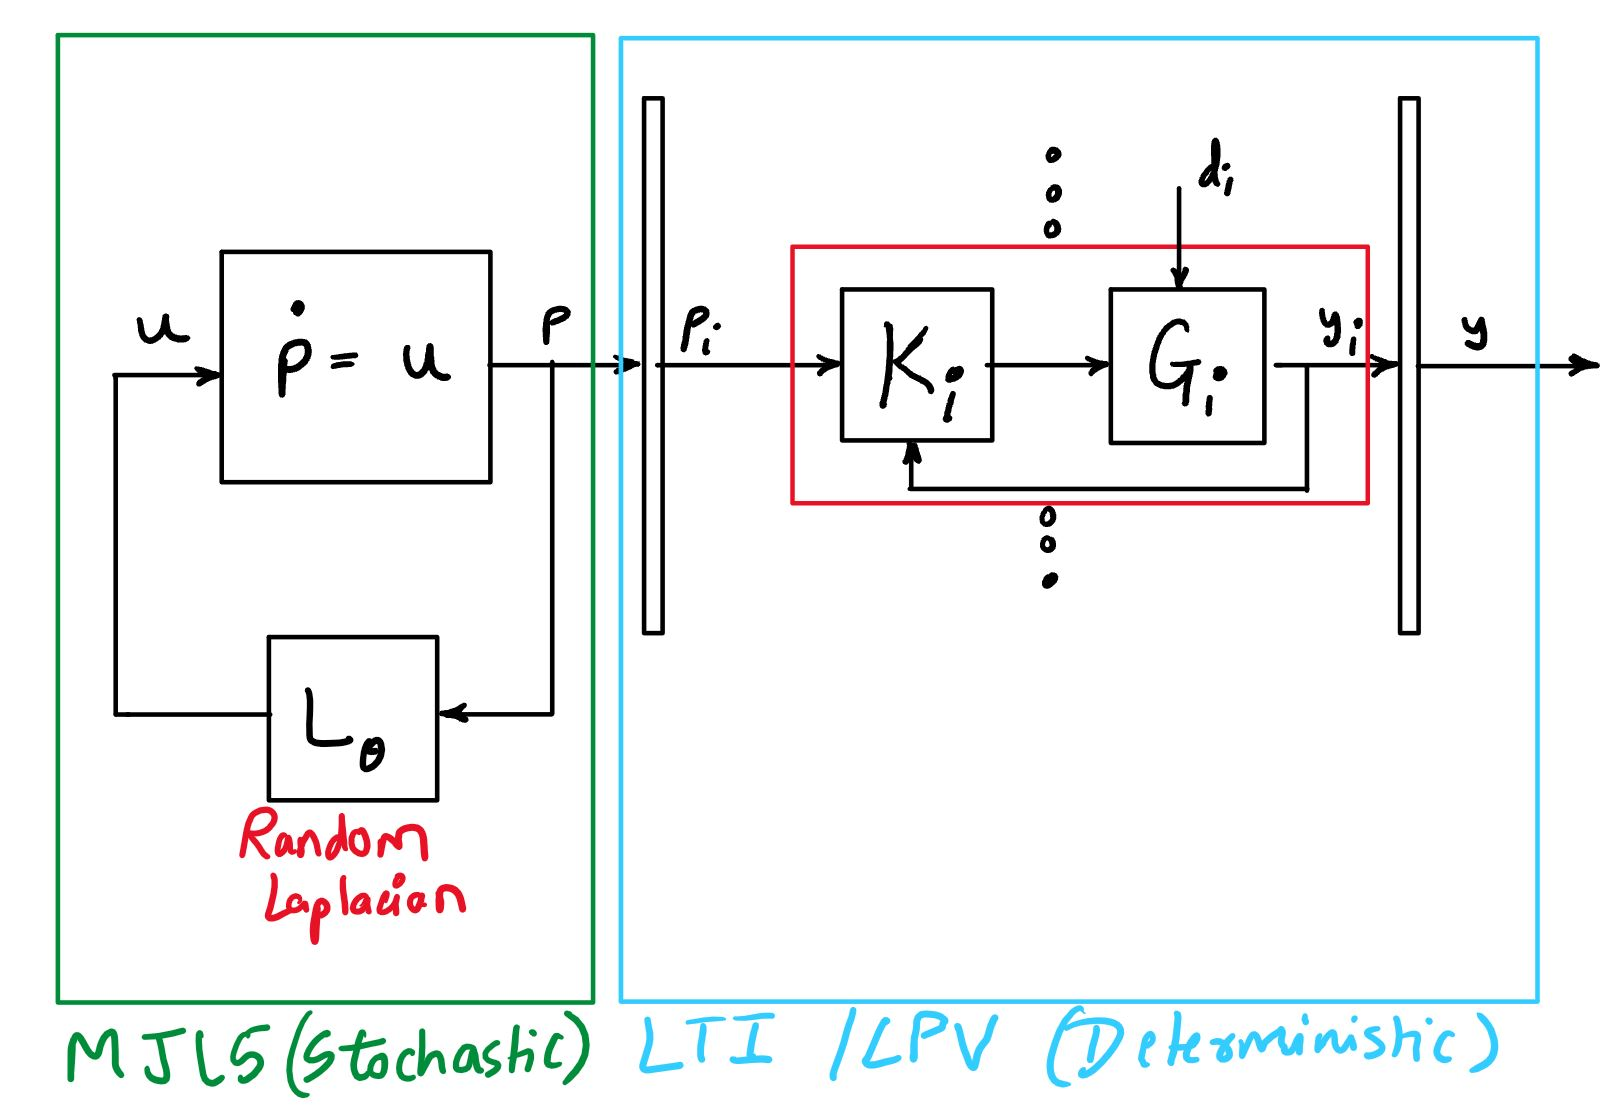
\includegraphics[scale=0.35]{figures/decoupled_stoch_deterministic.JPG}	
		\label{fig:Coupled}
	\end{figure}
	\begin{itemize}
		\item Model the Information flow dynamics as a Markovian Jump Linear System(MJLS)
		\item r2 or w2 measures (Daniel will talk more about this)
		\item IQC analysis of consensus Dynamics \footnote{Rantzer, 2016} -> Scalable condition
	\end{itemize}
\end{frame}